\documentclass[smallextended]{svjour3} 

%opening
\usepackage{times}
\usepackage{enumitem}
\usepackage{graphics}
\graphicspath{{Users/wafajohal/Dropbox/WRITING/MonThese/Figures/}{Users/wafajohal/Dropbox/WRITING/MonThese/Figures/illustrate/}{Users/Users/wafajohal/Dropbox/WRITING/MonThese/Figures/plots/}}
\usepackage{hyperref}
\usepackage{graphicx}  
\usepackage{subfigure} 

\begin{document}
\title{Behavioural Styles in Child-Robot Interaction%\thanks{Grants or other notes
%about the article that should go on the front page should be
%placed here. General acknowledgments should be placed at the end of the article.}
}
\subtitle{Do you have a subtitle?\\ If so, write it here}

%\titlerunning{Short form of title}        % if too long for running head

\author{First Author         \and
        Second Author %etc.
}

%\authorrunning{Short form of author list} % if too long for running head

\institute{F. Author \at
              first address \\
              Tel.: +123-45-678910\\
              Fax: +123-45-678910\\
              \email{fauthor@example.com}           %  \\
%             \emph{Present address:} of F. Author  %  if needed
           \and
           S. Author \at
              second address
}

\date{Received: date / Accepted: date}
% The correct dates will be entered by the editor
\maketitle
\begin{abstract}
	In this paper we present the concept of behavioural style as a tool for personalisation of robot's behaviour in specific roles. 
	We propose a study for which we have employed various kind of metrics to evaluate the perception and the influence of a robot's behavioural style on children. 
	This within subjects experiment took place in a smart apartment equipped with cameras, microphones and kinect sensor. 16 children from 7 to 11 participated to the experiment.
	In the experiment the robot would either have an authoritative attitude or a permissive attitude. 
	We measured the influence of this attitude via various medium:
	interviews of children, questionnaires, task performances, parents observation and confrontation, and postural analysis. 
	We show that postural analysis gave the best measure to predict the style of the robot from the child's point of view.
	These results illustrate recent tendencies in HRI to go away from self-assessment measures with young children.
\keywords{First keyword \and Second keyword \and More}	
\end{abstract}

%*****************************************************************************************************
\section{Introduction}
\label{sec:introduction}
%paragraph1 : general prgagraph about context 
As technology develops, there is a tendency of the multiplication of the numerical platforms in home-environments. 
The new dynamic of the Internet-Of-Things and connected objects have accelerated this phenomenon. 
Computer devices, tablet or cellphone users haven't yet established a social relationship with them. 
Creating a social relationship with the numerical devices could help increase trust and quality of life of individuals.
Where the users used to see these platforms as tools, they should now be able to exploit these artificial entities and create a social relationship that is trustable, controllable and credible. 
To this end, this user-tool relationship should evolve into a user-companion relationship, in which the user can count on his companion to care, help and entertain him.

Human-human communication is a large detailed field of study. 
Some signals sent between human interlocutors are subconscious while still having been processed by their cognition.
Subconsciously, humans emit social signals that shows their intentions and their goals.
These abilities are parts of what is called the social intelligence.
Several research fields, from human-computer interaction, affective computing, social signal processing, human-robot interaction, human activity recognition etc. are now working on enabling new technologies with social intelligence in order to make them more user-friendly and acceptable.
Researchers in HRI~\cite{Tapus2007,Dautenhahn2007} have also noted that robots need not only to be competent in the task but also socially intelligent.

%traditionally
Researchers in Human-Robot Interaction (HRI) have agreed that acceptability in home environments will come only via sociability\footnote{\textit{\textbf{Sociability} is the ability to perceive, understand and express social cues of communication in a human-understandable way.
It is also the ability to create and maintain social relationships; the ability to learn and develop social competencies }\cite{Dautenhahn2007}.} of the robots.


%our vision
The underlying assumption of this work is that the social personalisation of the companion's robot behaviour improves the acceptability of the users.
The interest in the personalisation of companion robots comes from the assumption that users want a more socially intelligent robot while keeping a certain controllability of their home assistant.
It is also assumed that social robots should display comprehensive behaviours for the user - in its decision and expressions.
For this, its reasoning processes should be made explicit to the user providing a level of understanding. 
Customisation of the behaviours on the other hand can improve the user's feedback as well as the controllability of his companion robot.
The perspective taken in this thesis is to propose a way for the user to chose the manner their companion robot would behave. 
This aims to contribute in both acceptability of the companion and to make the relationship and social bounding easier with the companion. 
In particular, the goal for this thesis is to investigate how the personalisation of the social robot's behaviour in context based on \textit{style} can be designed and evaluated in a realistic context and can contribute to \textit{social adaptability} of the companion robot's behaviour.

The challenge of the social adaptability of a robot's behaviour can be approached from different perspectives. 
The design of companion robots requires an understanding and a model of the \textit{plasticity} as well as reasoning and developing communicating vector of this adaptation. 
Our work takes concepts from several disciplines, aiming to benefit from various approaches of plasticity.
As the research went along, this work used notions from socio-psychology, cognitive sciences, artificial intelligence and affective reasoning, human-machine interaction, computer sciences and human-robot interaction.

From a more technical point of view, the variations in the ways social roles that a social robot  has to play can be seen as styles applied to a predefined script.
The notion of style and social role are important in this thesis: the robot plays a social role with a particular style in order to fit  the social expectations of the user better.
A social role is understood as a set of abilities, goals and beliefs of the robot and the style as a way of performing the social role.

%could ...

%research questions
\paragraph{research questions}
\begin{itemize}[noitemsep,nolistsep]
	\item Why should companion robots have styles ? (Section \ref{sec:soa_styles} )
	\item What distinguishes our approach from existing approaches for personalisation? (Section \ref{sec:soa_styles})
	\item Given the physical constraints of the robots (e.g., velocity limits, variation in mechanical degrees of freedom), how can this personalisation be carried out?(Chapter \ref{cha:stylemode})
	\item Can styles (parental) expressed by robots be recognized by parents ? (Chapter \ref{cha:evalonline})
	\item What is the influence of styles on the children's behaviours? (Chapter \ref{cha:stylebotxp})
	\item How can we measure the attitude changing in an interaction with a social robot? (Section \ref{sec:soa_nv})
	\end{itemize}

%paragraph 2 others, .... last sentence but pb

%paragraph 3 : In this paper we propose ...
contrary to prior work
we then evaluate
we then introduce
we compare
we show that
we also present resulst from experimental analysis indicating that 
findings from ... test indicate  statistically significant differences un 

additionally

finally we posited that even 
we conducted a follow up experiment to test this hypothesis

in section ... we discuss examples that motivate our work and place it in the context of other related work
Section 5 introduces

Section 7 presents 

We also discuss the applicability of the proposed metric of ... to ...
Finally, we describe an additional experiment designed to assess the benefit of ... in section 8.

We conclude with recommendations for the direction of future research in Section 9.

In this paper, we describe a user experiment aiming to investigate the influence of behavioural styles displayed by a humanoid robot on the perception and the attitude of a child in interaction with this robot. 
The experiment was conducted in the smart apartment Domus\footnote{Domus is an experimental platform composed especially with a domotic apartment \url{http://domus.liglab.fr/}} at the LIG Laboratory, equipped with camera sensors, microphones and other sensors and connected objects. 


%*****************************************************************************************************

\section{Related Literature/Work}
Context social adaptability

Personality matching
pb context independent

We would like a model to be context dependent


Style

\section{Style model}
Several expressibility parameters exist to characterise motion. 
We used some of these parameters to filter pre-designed motions and to generate \textit{style}d motion.

In the state of the art on styles in Psychology (in section \ref{ss:psychostyle}), we have differentiated cognitive styles (closer to the notion of personality) from other kinds of styles which are more role-dependent (such as leadership styles, parenting styles etc.).
Our definition of Behavioural Styles is in line with psychological role-dependent styles, and hence takes into account the role played by the robot.
Before giving details in the model and the generation process of \textit{style}d behaviour, let us clarify the properties of our behavioural styles:
\begin{center}
Behavioural Style Properties
	\begin{itemize}[noitemsep]
		%\item a way of playing a social role by a companion robot.
		\item described by a list of parameters
		\item expressed in non-verbal cues of communication
		\item associated to a meaningful concept in psychology
	\end{itemize}
\end{center}

%cf \cite{Dalle2012,Neff2008} for presentation of model and equation



\subsection{Design Approach}
In this section, the different modules involved in the style model are described. 
Then, we detail on the implementation and give some examples of style sheet and application on the Nao  and Reeti robots are given.

%\subsection{The context as a social role for the companion}
\subsubsection{Theoretical Grounding}
As presented previously, the \textbf{Plasticity} perspective is taken in order to render an adaptable companion robot.
Styles characterise the plasticity of the behaviour (variability in the same context) as opposed to the personality that characterises the behaviour consistency (consistency across contexts).
Our approach aims to apply plasticity concepts to HRI as it was applied in HCI. 

As described by \cite{Coutaz2012}, the context of use modelling, in which different styles can be applied is presented by the presence of three concepts :
\begin{itemize}[noitemsep,nolistsep]
\item the role: which corresponds to the social role for the companion robot.
\item the entities involved: corresponding to the number of robots involved and their competencies (role they can play).
\item the situational inter-relation: the listener, the speaker (one can also specify here the relative position of the agents).
\end{itemize}
Based on the previous study in Chapter~\ref{cha:explostudy}, we have identified 6 problems/situations for children alone at home and proposed 6 social roles for the companion robots to fulfil in these contexts.

Following the Scenario-based approach, (see~\ref{sec:senarbasedapp}), we propose a scenario that incorporates all of the above problem/situations while highlighting the interactions between the companion agents and the child. 
It should be noted that a social role, for example that of a Teacher, can be deployed via one or many forms (e.g. virtual agents and/or robotic agents) that will collaborate and cooperate in order to accomplish the tasks and to reply to the needs of a specific problem/situation.
An example of a scenario written in natural language can be found in the the Annex~\ref{annex:scenarMOCA}.




\subsection{Personalisation with Styles}
On top of the roles, behavioural styles, as previously mentioned, will affect the non-verbal expressibility within the role.

The notion of style is in this model: a set of behavioural changes that can be applied to any motion of a role repertoire and that leads to a meaningful interpretation of the way the motion is executed. 
A styles filter is used to generate behaviours according to the role and to the user's preferences. 
Only a few styles have been implemented for our experiments but the solution that we propose can be extended.
The aim is that users could choose the styles from a catalogue and set the one they prefer, providing hence the adaptability of the companion within the social role. 

As for CSS, the aim in the style framework for design of social behaviour for robots is to make them \textbf{reusable }and \textbf{flexible}.
We intent then to show that styles can be applied to various gestures and pre-defined behaviour but also used for various robotic platforms. 

The style model acts similarly to a filter. 
It is fed by neutral gestures that are contained in the role repertoire and applied at run-time on the pre-selected gesture. 
The stylized gesture is then sent to the scheduler in order to perform it.

The figure \ref{fig:workflowstyle} shows the general data work-flow for the runtime generation of stylistic motion.

Our system takes as input a pre-defined motion that has been selected to be performed. 
This motion belongs to a motion repertoire that is associated to the current role played by the robot.
The input \textbf{motion} is defined by a series of key-frames.
A motion is hence a tuple containing : 
the names of the joints active during this motion,
for each joint the list of relative \textit{time} when a key-frames appends and
for each joint and each time the associated \textit{key-frame} value (either angular or relative activation of the joint).

The styles are defined within the \textbf{Behavioural Style Sheet} (BSS) format. 
The style is set before run-time. 
It defines the modification that will be applied to the original motion.
The BSS is divided in two main parts, the hearer and the speaker parts.
Indeed,  according to the fact that the robot is reacting to someone speaking or speaking itself, the style parameters may vary.
The BSS is further discussed in the section \ref{ssec:bss}.

The \textbf{Style filter} is the core program written in Python. 
It contains some transformation algorithms inspired from works in 3D animation allowing the interpretation of the BSS and the generation of new motion.
Some examples of algorithms implemented in the current version of our system are presented in section \ref{sec:examples-of-stylized-motions}.
The generated motion can be however out-passing the physical constraints of the robot's motor. 

The \textbf{Post-Processing} module takes as input the platform's limits (speed and angular limits of each joints) and the generated motion and ensures that the computed styled motion is within these limits.
If not, the generated motion is modified to fit within the joints' constraints


%%todo \cite{Ruttkay1998} contraint based key-framinig As used in web-design to implement style, we propose a similar syntax to define styles within what we call Behavioural Style Sheet.

\subsection{Style filter}
\label{ssec:bss}
We defined behavioural styles according to the 1) static and 2) dynamic parameters, as well as 3) decorators patterns. 
These parameters allow us to depict variation of execution of motions.
The values taken by these parameters are referred to psychological models of style and are used as a percentage of the total value in order to be applicable to several platforms or the frequency rate.
\begin{figure}
	\centering
	%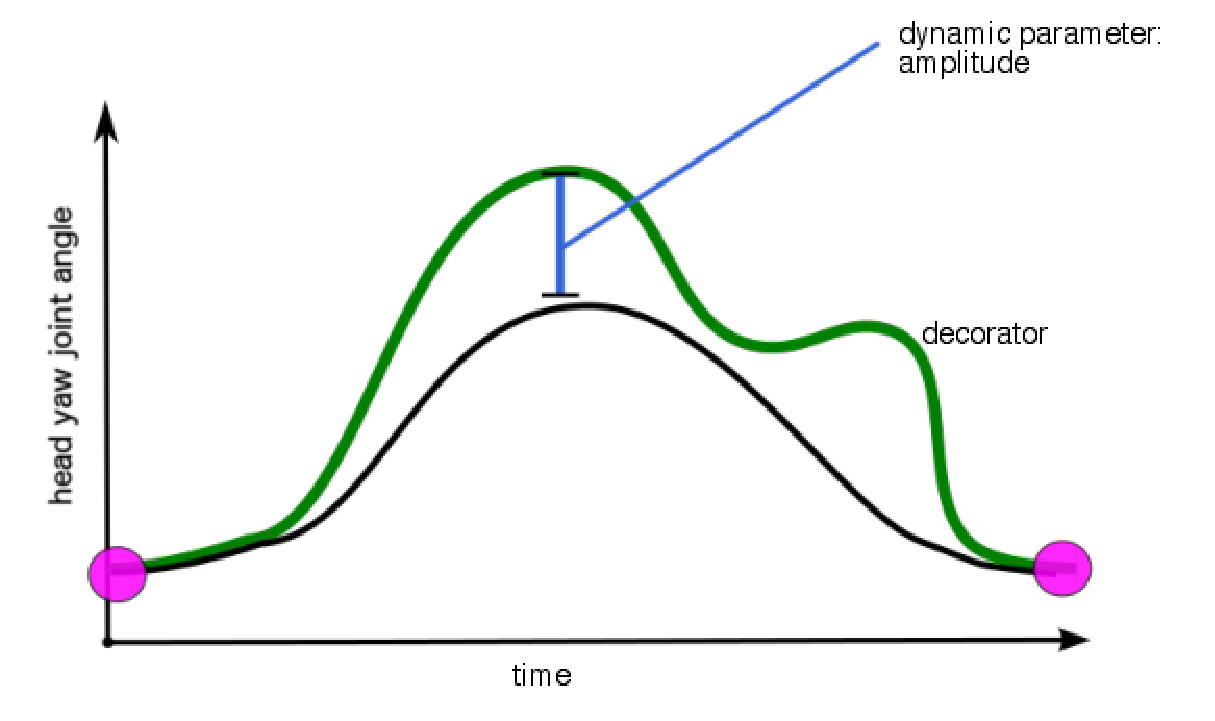
\includegraphics[width=0.8\linewidth]{style_graph}
	\caption{Style parameters for Head Yaw(green is stylized motion, black is original, the P0 pose is in pink)}
	\label{fig:styles_parameters}
\end{figure}

Figure \ref{fig:styles_parameters} shows an example of stylisation of a head yaw joint angle motion.
In this example, the static parameters are included in the $p0$ position.
The amplitude change is a part of the dynamic parameter. 
Finally the decorator is an additional keyframe with a new value. 
The decorator is often an additional motion that is fused with the current motion.

\paragraph{(1) Static parameters} allow to describe the neutral pose \texttt{p0}. 
This neutral pose \texttt{p0} is the posture the robot will take by default.
Sometimes, some joints of the body won't be in motion,  and hence the robot will keep the joint values of \texttt{p0}.
As before, we define this pose in accordance with the styles found in the literature. 
There are several static parameters that exist to describe poses. 
\texttt{p0} is very platform dependent. 

The definition of the pose is made in a specific file for each robotic platform.
Figure \ref{fig:p0} shows an example of the call of the \texttt{p0} poses as defined for the Authoritative and Permissive styles for the Nao robot. 
The style modeller makes a reference to this file in order to build the stylized motion at runtime and adds p0 before and after each motion event to ensure that it is the default pose.




\paragraph{(2) Dynamic parameters}
From the literature in HRI and virtual agents in the domains of animation and psychology, we have listed some dynamic parameters that can be useful to depict changes in styled motion.
The current implementation of styles take into account the following parameters. 

\begin{itemize}[noitemsep,nolistsep]
	\item Amplitude: the spacial extent related to the dimension of expansiveness from Gallaher and Meharbian.
	\item Speed: temporal extent and the velocity of execution of the movement.
	\item Tempo: specifies a rhythm for the key-frames in the motion (that are spaced according to the tempo).
	\item Noise: opposed to fluidity, noise makes the movements jerky where smoothing makes the movement fluid.
	\item Duration: specifies a duration for the motion.
\end{itemize}
These parameters are set for each style, and for each of them, an algorithm takes the current motion and the value of this dynamic parameter to compute a new motion.
For instance, one can double the amplitude, change the rate, add a tempo to the motion and make the motion noisy.
An example of dynamic parameters in the BSS is given in figure \ref{fig:dyna}.


The Algorithm \ref{algo:speed} gives the method to compute new times for the keyframe for each joint with a certain magnitude change.
In this algorithm, we first compute the duration between the time of the current keyframe and the time of the previous keyframe. 


\section{Research Questions and Scenario}\label{sec:research-questions-and-scenario}
After the on-line study (Chapter \ref{cha:evalonline}), this experiment aimed to do a real user experiment in an ecological environment in order to test the credibility and the acceptability of styles by children. 

One of the research questions behind the experiment was to test the style model and the plasticity model of the companion proposed in Chapter \ref{cha:stylemode} and \ref{cha:caio}. 
In a social relationship, the perceived signals are encoded, and each of the partners influence the thinking and the actions of the other.
This influence can be subconscious and very tricky to identify. 
Phenomena such as synchrony and imitation can be observed. 

%This experiment as to not rely only on subjective data but also tried to measure objectively the change of behaviour of the children according to the style or versatility of the robots.
In this experiment, the same styles - Authoritative and Permissive -  as the ones were applied to the robots previously (Chapter~\ref{cha:evalonline}) were used.
From these previous results, Authoritative and Permissive styles seemed to be identifiable by parents and applicable on the two robots Nao and Reeti. 
These styles were also in line with the psychological dimensions of parenting styles. 
The results on credibility also showed that styles could be an interesting factor to take into account. 

With this experiment, we wanted to verify our plasticity framework applied to HRI in a more general manner. 
In that sense, this experiment was also questioning versatile vs specialist robots. 
The aim here was to collect opinions of parents and children on the versatility of a companion robot and see if it was preferable to have a companion robot able to play several roles or does it affect its credibility and trust in accomplishing the tasks to be versatile.

In the experiment scenario, the child alone at home has to review his multiplication tables. 
His Teacher companion is here to ask him questions and to check if he knows them. 
After some questions, the companion(s) propose to dance for the child (faking that it has a dance competition) taking the Buddy role. 
However, some more questions of the math quiz have to be answered by the child and the companion retakes the Teacher role.


\section{Method}
\subsection{Hypothesis}
%Todo here reading the chap7}
Following are a list of our principal hypothesis :
\begin{itemize}[noitemsep,nolistsep]
	\item[H0] Authoritative robots are perceived to be more dominant than permissive by children.
	\item[H1] Styles influence children's engagement in an interactive task.
	\item[H2] Styles influence the perceived competence and credibility of the robot in an interactive task.
	\item[H3] Styles influence the complicity with the robot in an interactive task.
	%\item[H4] Versatility of a companion increases the attachment and engagement of the children in interaction with it.
	\item[H4] Role-Specialist robots are perceived to be more competent and trustworthy than versatile robots.
	%\item[H6] There is an influence of the style during the math quiz during the dance on the child's behaviour.
\end{itemize}

\subsection{Subjects/Participants}
Ethical validation has been obtained from the CNIL and CERNI.
It enabled us to prepare an Information Notice and a Consent Form for parents and children participating to the experiment.
The recruitment was done within the researchers of the laboratories of Grenoble area. 
Parents were either staff members of the administration or the researchers at the laboratory.
We recruited voluntary parents and children during a period of 2 weeks preceding the experiments. 
The experiment took place during winter holidays. 
16 children participated to the experiment with ages from 


\subsection{Apparatus/Materials}
\subsection{Design}
\subsection{Procedure}
The protocol has been established in collaboration with the PIMLIG.
Ethical  validation has been obtained from the CNIL and CERNI.
It enabled us to prepare an Information Notice (see Annex \ref{ann:noticeinfo}) and a Consent Form  (see Annex \ref{ann:consentement}) for parents and children participating to the experiment.
The recruitment was done within the researchers of the laboratories of Grenoble area. 
Parents were either staff members of the administration or the researchers at the laboratory.

\subsubsection{The Domus Experimental Platform and Sensors}
The experiment took place in an ecological environment at Domus.
Domus is an experimental platform of the LIG Laboratory. 
The Figure \ref{fig:domus3d} shows the map of Domus.
%\begin{figure}[h]
%	\centering
%	\includegraphics[width=0.8\linewidth]{Domus_def2}
%	\caption{Domus Experimental Platform}
%	\label{fig:domus3d}
%\end{figure}
Domus is composed of several rooms, or physical spaces:
\begin{itemize}[noitemsep,nolistsep]
	\item A fully equipped and functional apartment composed of:
	\begin{itemize}[noitemsep,nolistsep]
		\item a kitchen
		\item an office/living-room (where the experiment took place)
		\item a bedroom (where the interviews of the children took place)
	\end{itemize}
	\item A sound and video direction room, from where one can access audio and video capture in the apartment and record from the control PCs
	\item An open space divided into a meeting/video-conference room and a common area.
\end{itemize}

The Figure \ref{fig:domusroof} shows the experimental settings in the living room. 
The grey window is a tainted-window (with the green star). 
We added a Kinect sensor (yellow star) and a wooden board on the floor to avoid the robot falling. 
%\begin{figure}[h]
%	\begin{tabular}{c c}
%	%	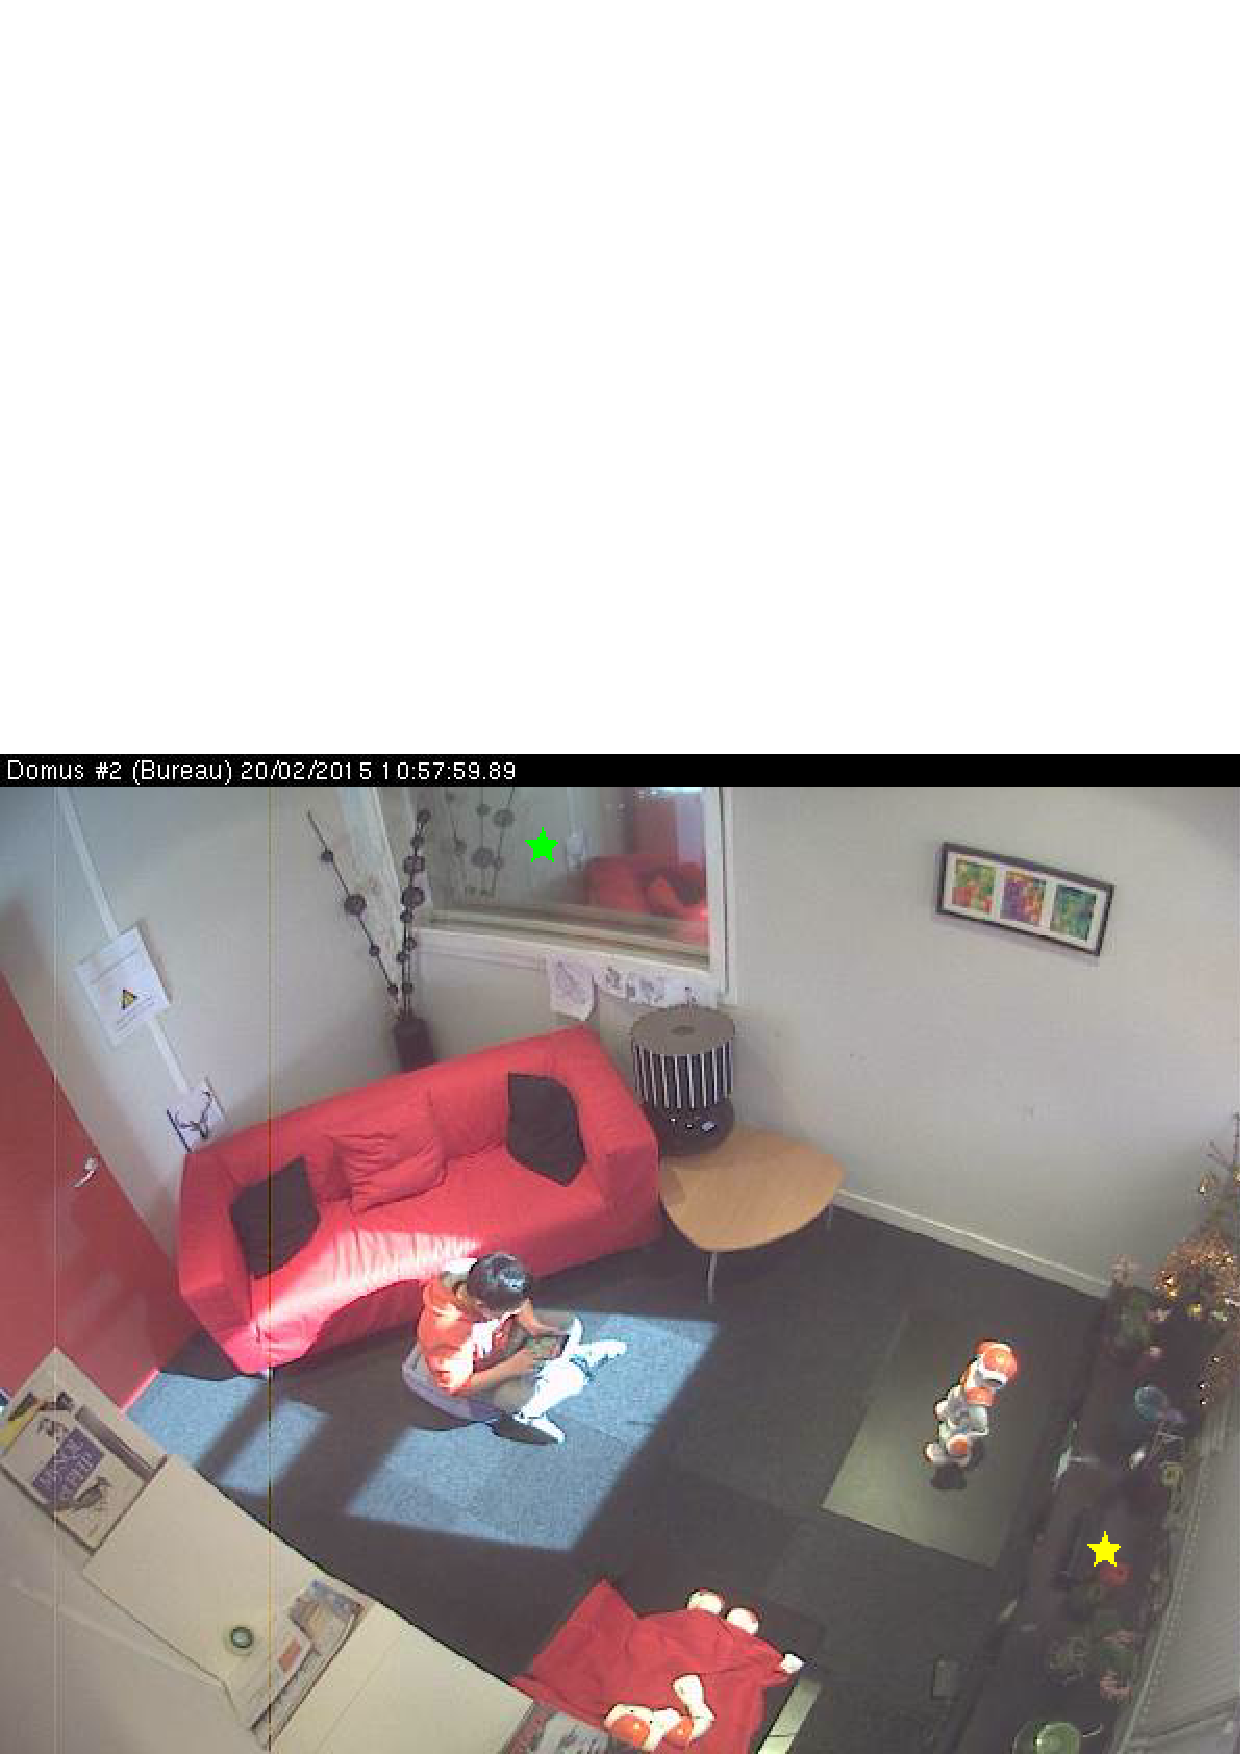
\includegraphics[width=0.45\linewidth]{illustrate/roof1.png}&
%	%	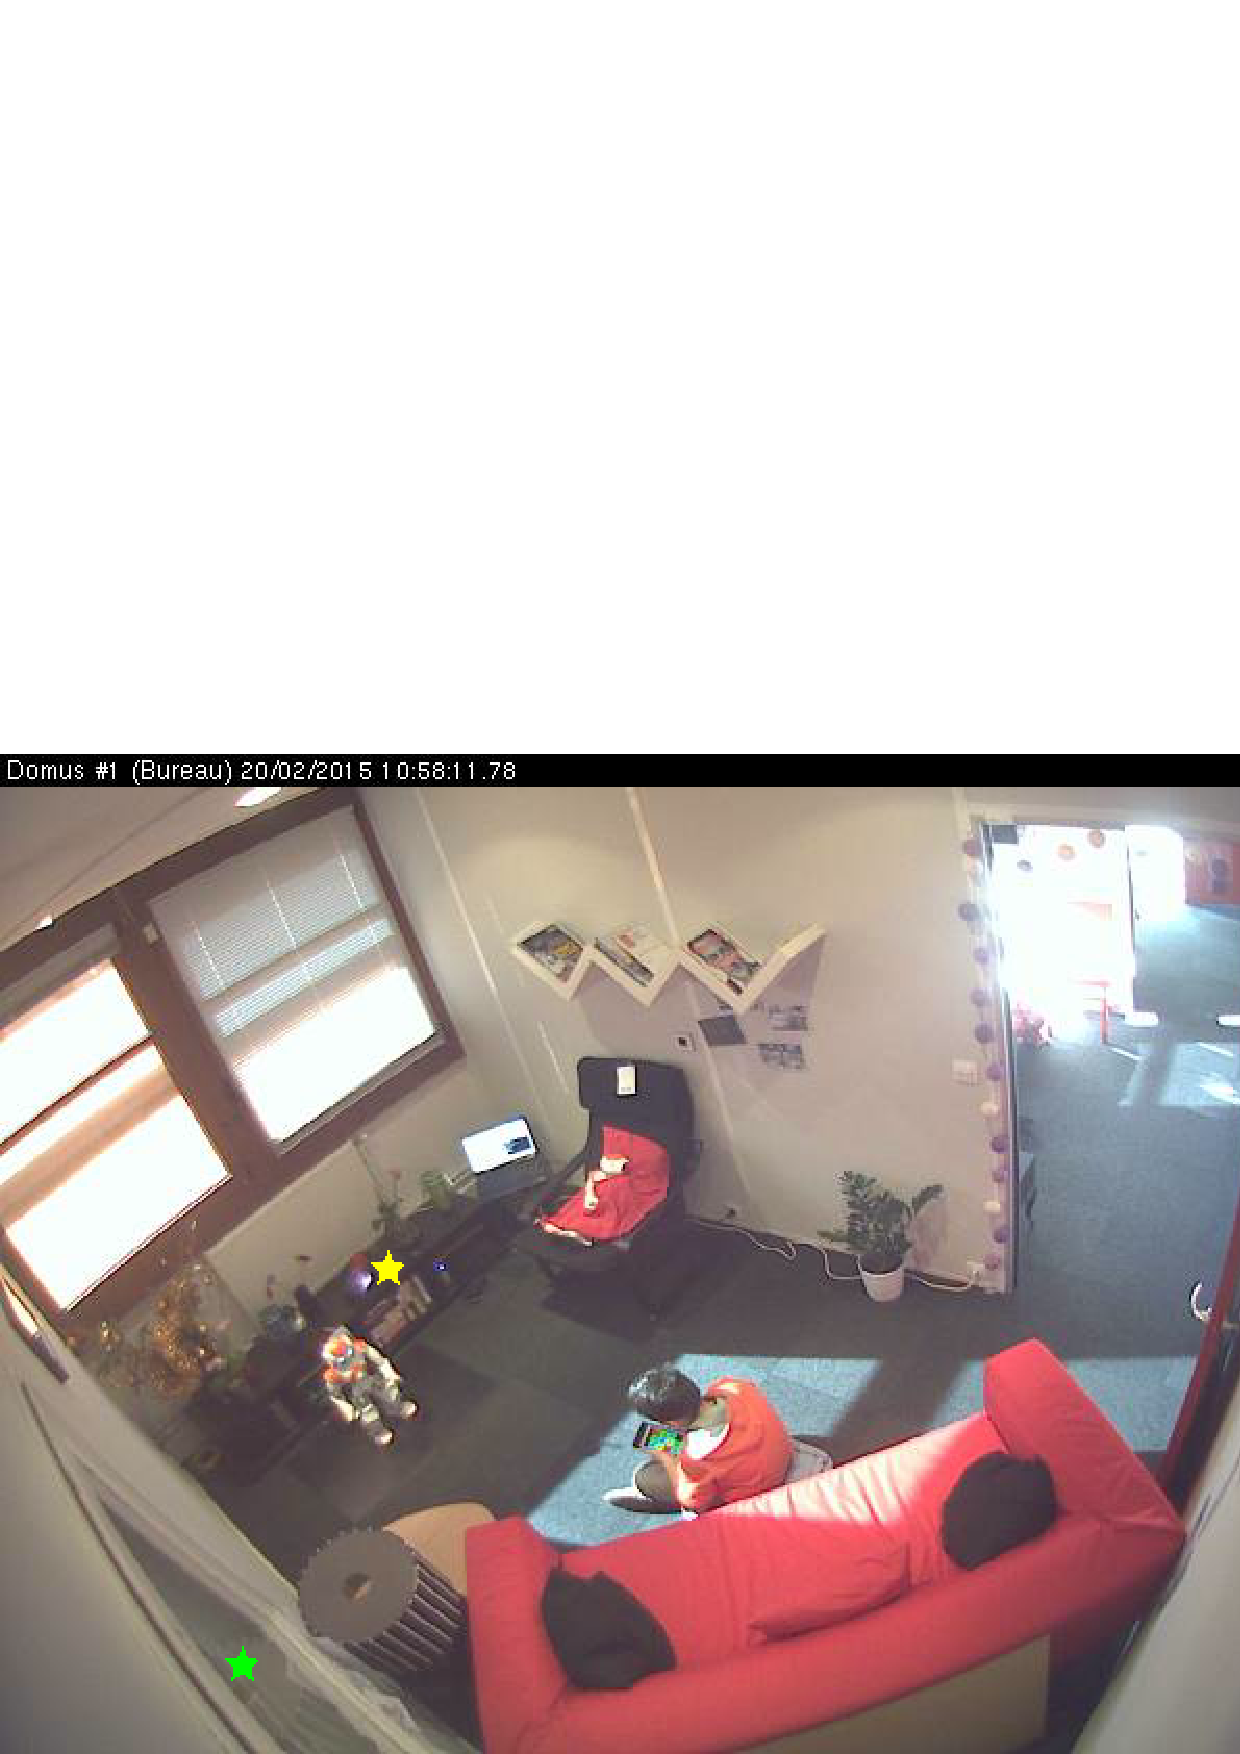
\includegraphics[width=0.45\linewidth]{illustrate/roof2.png}
%	\end{tabular}
%	\caption{Experimental Settings}
%	\label{fig:domusroof}
%\end{figure}
%The Domus apartment is controllable by the OpenHab\footnote{\url{http://www.openhab.org}} middle-ware. 
OpenHab is a home control middle-ware that supports various sensors, protocols and operating systems. 
We were able, for instance, to launch music playback on the speaker of the apartment directly form the robot, by doing a simple HTTP\_REQUEST. 

\subsection{Measures}
\section{Results}
\section{Discussion}
\section{Conclusion}

%Statistics
%ANOVA results are cited using the F test (e.g., $F (1, 38) = 4.94$, $p = .04$). F and p are italicized. Give the exact $p$ value to two decimal places except when greater better than $p < .01$. Try to avoid more than two decimal places, as readers are not very interested in exact values; comparisons are more important. The $F$ value is followed by the degrees of freedom in the numerator and denominator. Here is how one author of a mobile phone study (Author, 2010) reported an interaction effect:
%\begin{quotation}
%The data were analyzed in a 2 (Age: young vs. old) x 2 (Device: Phone A vs. B) mixed measures analysis of variance (ANOVA). We found an interaction of Age X Phone ($F [1, 38] = 26.18$, $p < .0001$). The contrast showed older people using Phone B took considerably longer to complete the task, $F (1, 38) = 69.16$, $p = .02.$ (p. 6).
%\end{quotation}
%Correlations using product moment tests are reported using $r$ (e.g., $r (200) = .19$). The number in parenthesis following the $r$ value represents the degrees of freedom ({\it df}),  or N Ð 1. Including the degrees of freedom provides the reader with a sense of statistical significance, in that correlations are highly sensitive to the number of data points. For instance, with 200 scores on both variables, .19 will be a significant correlation whereas with only 30 people, it will not be statistically significant.
%
%T tests (e.g., $t [20] = 100.2$, $p < .01$) are reported giving the degrees of freedom in the denominator. (The numerator {\it df} is always $1$, as is true of correlations.)
%Notice how brackets are placed inside parentheses to reduce confusion.

%*****************************************************************************************************


%*****************************************************************************************************



\section{Table of Behaviours for each style factor from \cite{Gallaher1992}}
\label{tab:styledims_gallaher}
\begin{table}[h]
	\small
	\centering
	\begin{tabular}{|l |c|  l |}\hline
		\textbf{Behavioural Items}  &	\textbf{Style factor} & Computationable term \\ \hline
		Uses very little-most of body when gesturing & Expressiveness  & TODO \\
		Slow-fast gestures  & Expressiveness & Velocity \\
		Gestures: infrequently-frequently & Expressiveness & QOM\\
		Shakes head: frequently-rarely & Expressiveness &  head motion and head angular velocity in 3D\\
		Narrow-broad gestures & Expressiveness & Extensiveness \\
		Nods head: frequently-rarely & Expressiveness & head motion and head angular velocity in 3D \\ \hline
		
		Shoulders: slumped-erect when standing & Animation & shoulder opening angle\\
		Sits down and stands up: slowly-quickly & Animation & TODO\\
		Torso: upright-leaning when standing & Animation & torso lean angle\\
		Sits with torso: tilted-vertical & Animation & todo\\
		Slow-fast walker & Animation & none\\
		Sits with torso: erect-slumped & Animation & todo? \\ \hline
		
		Legs: together-wide apart when sitting & Expansiveness & legs extensivess\\
		Soft-loud voice & Expansiveness\\
		Elbows: close to-away from body & Expansiveness & elbows distace to core\\
		Thin-full voice & Expansiveness\\
		Light-heavy step & Expansiveness\\
		Takes: small-large steps & Expansiveness\\
		Legs: close together-wide apart when standing  & Expansiveness\\
		Hands: close to-away from body & Expansiveness \\ 
		Soft-loud laughter & Expansiveness\\ \hline
		
		Choppy-rhythmic speech & Coordination\\
		Jerky-fluid walk & Coordination & jerkiness\\
		Rough-smooth gestures & Coordination\\
		Harsh-smooth voice & Coordination\\ \hline
		
	\end{tabular}
	%\caption{Table of Behaviours for each style factor from \cite{Gallaher1992}}
	
\end{table} 




\section{Acknowledgements}


\section{Biblography}
\bibliography{jhri16.bib}


\end{document}
